\section{Implementation of \method{}}
\label{app:implementation}

Figure~\ref{fig:tisd-pseudocode} summarizes the branch--regenerate--distill procedure of \method{}, using the self-distillation objective of SDPO~\citep{hubotter2026sdpo}.

\begin{figure}[ht]
  \centering
  \begin{tcolorbox}[colback=CodeBackground,boxrule=0pt,arc=2mm,left=22pt,right=8pt,top=7pt,bottom=7pt]
\begin{lstlisting}[style=tisd-pseudocode]
def tisd_step(prompts, student, teacher):
    # 1. Sample responses, verify, and build privileged contexts.
    batch = collect_rollouts(student, prompts)
    retained = []

    # 2. Retain original trajectories; regenerate eligible failures.
    for x, y, reward, c in batch:
        z = y
        if reward == 0 and eligible(y, c):
            t = peak_divergence_pos(student, teacher, x, y, c)
            token = teacher.argmax(x, y[:t], c)
            prefix = y[:t] + [token]
            z = prefix + student.generate(x, prefix)
        retained.append((x, z, c))

    # 3. Distill the retained trajectories.
    loss = distillation_loss(student, teacher, retained)
    student.update(loss)
    teacher.update_ema(student)
\end{lstlisting}
  \end{tcolorbox}
  \caption{\method{} pseudocode. Each record contains a prompt \texttt{x}, response \texttt{y}, binary reward, and privileged context \texttt{c}. \texttt{peak\_divergence\_pos} selects the eligible position with the largest teacher--student divergence. Loss and optimization settings appear in Appendix~\ref{app:hyperparameters}.}
  \label{fig:tisd-pseudocode}
\end{figure}

\section{Preliminary Analysis: Full Details}
\label{app:analysis}

This appendix provides the full diagnostic analysis supporting \method{}'s branch selection and regeneration design (Section~\ref{sec:analysis}). The source trajectories come from SDPO training of Qwen3-$\{$1.7B, 4B, 8B$\}$~\citep{yang2025qwen3} on LiveCodeBench v6~\citep{jain2024livecodebench}; a typical training step collects $256$ rollouts ($32$ problems $\times$ $8$ rollouts). We focus on failed rollouts because \method{} branches from them and because they allow us to examine the teacher guidance available beyond the original student trajectory. We first describe the analysis protocol, then provide additional breakdowns of the diagnostics in Section~\ref{sec:analysis} and extend the intervention analysis to other architectures and science domains.

\subsection{Analysis Protocol}
\label{app:eval}

The coding diagnostics combine semantic annotation with execution-based evaluation. For semantic annotation, GPT-5.4 (temperature $0$, $1024$ completion tokens) receives the problem statement, the student's full solution, and a $15$-token context window centered on the selected position, and classifies both the student and teacher tokens by \emph{semantic role} (algorithmic, naming, formatting, non-code text).

For continuation evaluation, we preserve the student prefix before the selected position, force the teacher's argmax token, and greedily generate the suffix using either the teacher (\emph{teacher continuation}) or the student (\emph{student continuation}). The matched student control instead forces the student's original token before regenerating the suffix. On LiveCodeBench, the resulting Python block is extracted and executed against the full private test suite; a response is correct if and only if it passes all test cases.

On SciKnowEval L3, correctness is binary: the extracted answer option must exactly match the reference answer. We apply the same criterion to the original rollout and each regenerated continuation. The cross-domain analysis uses Qwen3-8B rollouts with $32$ problems and eight rollouts per problem in each science domain. Success rates are conditioned on original failures, and pooled science rates aggregate outcomes over all $553$ failed rollouts.

\subsection{KL Concentration CDF}
\label{app:kl-conc}

The KL concentration ratio $C = \mathrm{KL}(\tstar)/\sum_t \mathrm{KL}(t)$ measures the fraction of total response KL carried by the peak-divergence position. Figure~\ref{fig:concentration-cdf} shows its cumulative distribution across $202$ failed Qwen3-1.7B rollouts. The median concentration is ${\sim}19.5\%$, with $\tstar$ accounting for more than $50\%$ of total response KL in some cases. Across model scales, the concentration decreases from $19.5\%$ at 1.7B to ${\approx}9\%$ at 4B and 8B. Even at ${\approx}9\%$, the peak position carries roughly $40\times$ the per-position average KL.

\begin{figure}[ht]
  \centering
  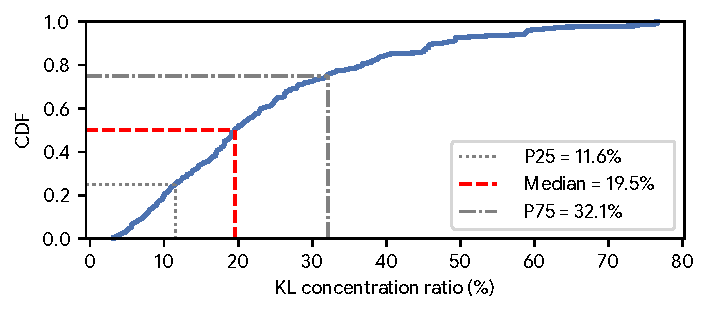
\includegraphics[width=0.6\linewidth]{figures/fig7_concentration_cdf.pdf}
  \caption{CDF of the reverse-KL concentration ratio $\mathrm{KL}(\tstar)/\sum_t \mathrm{KL}(t)$ on $202$ failed Qwen3-1.7B LiveCodeBench v6 rollouts.}
  \label{fig:concentration-cdf}
\end{figure}

\subsection{Semantic Role Breakdown}
\label{app:semantic}

Table~\ref{tab:semantic-role} reports GPT-5.4 semantic annotations of the student and teacher tokens at $\tstar$ on failed rollouts. At larger model scales, both student and teacher tokens at peak divergence are predominantly classified as non-code text, while algorithmic roles become less frequent.

\begin{table}[ht]
\caption{GPT-5.4 semantic annotations of student and teacher tokens at $\tstar$ on failed Qwen3-\{1.7B, 4B, 8B\} LiveCodeBench v6 rollouts. Entries are percentages within each model scale.}
  \label{tab:semantic-role}
  \centering
  \small
  \begin{tabular*}{0.7\linewidth}{@{\hspace{6pt}\extracolsep{\fill}}llccc@{\hspace{6pt}}}
    \toprule
    & Role & 1.7B & 4B & 8B \\
    \midrule
    \multirow{4}{*}{Student}
    & Algorithmic   & 36.1\% & 11.6\% & 11.6\% \\
    & Naming        & 11.4\% &  3.9\% &  5.5\% \\
    & Formatting    &  7.4\% & 13.3\% & 12.7\% \\
    & Non-code text & 45.0\% & 71.3\% & 70.2\% \\
    \midrule
    \multirow{4}{*}{Teacher}
    & Algorithmic   & 38.6\% & 10.5\% & 14.4\% \\
    & Naming        &  9.9\% &  4.4\% &  3.9\% \\
    & Formatting    &  8.4\% & 11.6\% & 13.8\% \\
    & Non-code text & 43.1\% & 73.5\% & 68.0\% \\
    \bottomrule
  \end{tabular*}
\end{table}

Figure~\ref{fig:transition-matrix} shows the student-to-teacher semantic-role transition matrix. The diagonal dominates across model scales, indicating that the student and teacher tokens at $\tstar$ often belong to the same broad semantic category. Thus, large teacher--student divergence frequently reflects differences within a semantic role, such as alternative variable names or different comments, rather than a change in the type of token being produced.

\begin{figure}[ht]
  \centering
  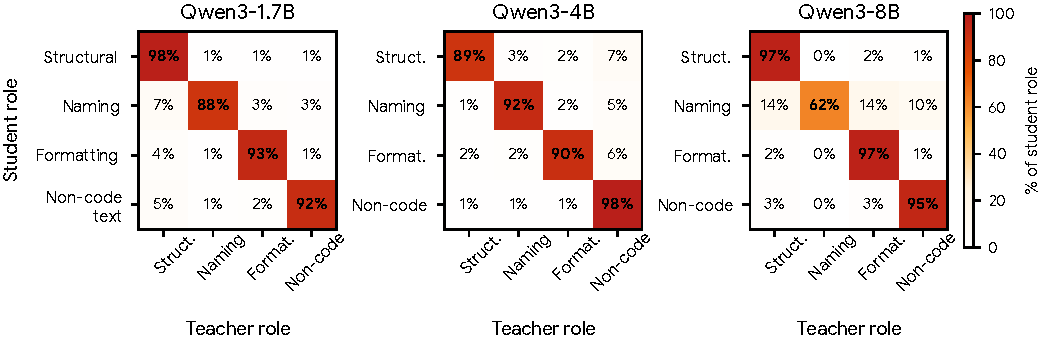
\includegraphics[width=\linewidth]{figures/fig_transition_matrix.pdf}
  \caption{Student-to-teacher semantic-role transitions at $\tstar$ on failed Qwen3-\{1.7B, 4B, 8B\} LiveCodeBench v6 rollouts. Each row shows the distribution of teacher-token roles conditioned on the corresponding student-token role. The dominant diagonal shows that disagreement usually remains within a semantic category.}
  \label{fig:transition-matrix}
\end{figure}

\subsection{Effect of Branch-Selection Position}
\label{app:branch-position}

Peak-divergence selection yields the highest student continuation success among the evaluated branch selectors on failed Qwen3-8B LiveCodeBench rollouts (Table~\ref{tab:steer_qwen8b_positions}). Forcing the teacher token at peak divergence gives $9.9\%$ success, compared with $6.1\%$ at first divergence and $1.7\%$ at random positions. The corresponding original-token controls yield $1.7\%$, $2.2\%$, and $3.3\%$, respectively. Teacher continuation shows a different ordering: first divergence reaches $17.1\%$, exceeding $13.3\%$ at peak divergence. Thus, the branch position that best supports student regeneration differs from that which best supports teacher continuation. Since \method{} returns suffix generation to the student, these results support peak divergence as its branch-selection criterion.

\begin{table}[ht]
  \caption{Effect of branch-position selection on $181$ failed Qwen3-8B LiveCodeBench v6 rollouts. Semantic roles refer to the student token at the selected position and are assigned by GPT-5.4. Execution success is measured after either teacher continuation or student regeneration from the forced teacher or original token. \emph{First divergence} denotes the first position where the student and teacher argmax tokens differ.}
  \label{tab:steer_qwen8b_positions}
  \centering
  \small
  \begin{tabular*}{0.82\linewidth}{@{\extracolsep{\fill}}llccc@{\hspace{6pt}}}
    \toprule
    & & Peak divergence & First divergence & Random \\
    \midrule
    \multicolumn{2}{l}{\textit{Semantic role ({student token at $\tstar$})}} \\
    & Algorithmic   & 11.6\% &  0.6\% & 20.4\% \\
    & Naming        &  5.5\% &  0.0\% &  3.9\% \\
    & Formatting    & 12.7\% & 15.5\% & 11.0\% \\
    & Non-code text & 70.2\% & 84.0\% & 64.6\% \\
    \midrule
    \multicolumn{2}{l}{\textit{Execution-based success rate at $\tstar$}} \\
    & Teacher continuation
      & 13.3\% & 17.1\% & 8.3\% \\
    & Student cont.\ (teacher token)
      & 9.9\% & 6.1\% & 1.7\% \\
    & Student cont.\ (original token)
      & 1.7\% & 2.2\% & 3.3\% \\
    \bottomrule
  \end{tabular*}
\end{table}
































\subsection{Persistence During Training}
\label{app:stepwise}

Non-code text remains the largest semantic category at peak divergence throughout Qwen3-1.7B SDPO training. Table~\ref{tab:stepwise} reports checkpoints from steps $0$ to $80$. Over this interval, the overall rollout pass rate increases from $0.211$ to $0.434$, while the algorithmic share of peak-divergence positions among failed rollouts decreases from $36.1\%$ to $26.2\%$. Semantic-role percentages are computed separately over the failed rollouts at each checkpoint.

\begin{table}[ht]
\caption{Evolution of rollout pass rate and semantic roles at the peak-divergence position during Qwen3-1.7B SDPO training on LiveCodeBench v6, using $256$ rollouts per update. Pass rate is computed over all rollouts, while GPT-5.4 semantic-role percentages are computed over failed rollouts at each update; the corresponding failure counts are shown in parentheses.}  \label{tab:stepwise}
  \centering
  \small
  \begin{tabular*}{\linewidth}{@{\extracolsep{\fill}}llccccc@{\hspace{6pt}}}
    \toprule
    & & \makecell{Step 0\\(202)} & \makecell{Step 20\\(183)} & \makecell{Step 40\\(192)} & \makecell{Step 60\\(176)} & \makecell{Step 80\\(145)} \\
    \midrule
    \multicolumn{2}{l}{Pass rate} & 0.211 & 0.285 & 0.250 & 0.312 & 0.434 \\
    \midrule
    \multicolumn{2}{l}{\textit{Semantic role ({student token at $\tstar$})}} \\
    & Algorithmic   & 36.1\% & 35.5\% & 36.5\% & 35.8\% & 26.2\% \\
    & Naming        & 11.4\% & 15.3\% & 12.0\% & 14.8\% &  9.7\% \\
    & Formatting    &  7.4\% &  8.2\% & 13.5\% & 11.4\% & 15.9\% \\
    & Non-code text & 45.0\% & 41.0\% & 38.0\% & 38.1\% & 48.3\% \\
    \bottomrule
  \end{tabular*}
\end{table}

\subsection{Contribution of Failed-Rollout Supervision}
\label{app:failed-supervision}

We ablate supervision on failed rollouts during Qwen3-1.7B SDPO training on LiveCodeBench. At step $80$, applying the KL loss only to successful rollouts yields $0.372$ validation accuracy, compared with $0.480$ when supervising both successful and failed rollouts, a difference of $10.8$ percentage points. This fixed-step comparison motivates analyzing the teacher guidance available on failed rollouts, which remain useful training examples under the standard SDPO objective.


\subsection{Cross-Architecture Validation}
\label{app:crossarch}

We replicate the Section~\ref{sec:analysis} diagnostic on OLMo3-7B-Instruct~\citep{olmo2025olmo3} at step $0$, using $221$ non-truncated LiveCodeBench v6 rollouts after excluding $35$ responses that reached the $16{,}384$-token limit. The main patterns observed with Qwen3 persist (Table~\ref{tab:olmo3}). On failed rollouts, non-code text accounts for $81.4\%$ of peak-divergence positions, and teacher continuation succeeds on $24.8\%$ of failures. The trajectory-steering effect also reproduces: forcing the teacher token and returning generation to the student yields $10.1\%$ success, compared with $6.2\%$ when retaining the original student token. Thus, the qualitative findings on peak-divergence semantics and teacher-guided student regeneration extend beyond the Qwen3 architecture.

\begin{table}[ht]
\caption{Reverse-KL diagnostic on $221$ non-truncated OLMo3-7B-Instruct LiveCodeBench v6 rollouts. Entries report semantic-role distributions at $\tstar$ and execution success after continuation from $\tstar$, separately for failed and successful original rollouts.}  \label{tab:olmo3}
  \centering
  \small
  \begin{tabular*}{0.6\linewidth}{@{\extracolsep{\fill}}llcc@{\hspace{3pt}}}
    \toprule
    & & \makecell{Fail\\(129)} & \makecell{Succ\\(92)} \\
    \midrule
    \multicolumn{2}{l}{\textit{Semantic role (student token at $\tstar$)}} \\
    & Algorithmic   &  7.8\% & 15.2\% \\
    & Naming        &  3.1\% & 10.9\% \\
    & Formatting    &  7.8\% & 10.9\% \\
    & Non-code text & 81.4\% & 63.0\% \\
    \midrule
    \multicolumn{2}{l}{\textit{Execution-based success rate at $\tstar$}} \\
    & Teacher continuation & 24.8\% & 69.6\% \\
    & Student cont. (teacher token) & 10.1\% & -- \\
    & Student cont. (original token) & 6.2\% & -- \\
    \bottomrule
  \end{tabular*}
\end{table}

\subsection{Cross-Domain Validation}
\label{app:crossdomain}

Teacher-token intervention also improves student continuation success on SciKnowEval L3 (Table~\ref{tab:tstar_fail_lcb_science_qwen8b}). Across $553$ failed Qwen3-8B science rollouts, student continuation from the teacher token succeeds on $39.4\%$, compared with $24.4\%$ for the original-token control, with the improvement appearing in all four domains. The corresponding LiveCodeBench rates are $9.9\%$ and $1.7\%$. Teacher continuation itself is substantially more successful on science, reaching $93.5\%$ compared with $13.3\%$ on coding failures. These results show that teacher-selected branch actions improve student continuation across both task settings, while the teacher's ability to complete the trajectory differs substantially between science and coding.

\begin{table*}[ht]
\caption{Verifier-based intervention on failed Qwen3-8B SciKnowEval L3 rollouts at SDPO update 0. The teacher is conditioned on the first successful same-problem rollout in source order, excluding the target rollout, and $\tstar$ is the valid response position with maximum reverse KL. Each domain contains $32$ problems with eight rollouts per problem. Numbers in parentheses denote failed-rollout counts.}  \label{tab:tstar_fail_lcb_science_qwen8b}
  \centering
  \small
  \setlength{\tabcolsep}{3.5pt}
  \begin{tabular*}{\textwidth}
    {@{\extracolsep{\fill}}llccccc@{\hspace{6pt}}}
    \toprule
    & & \makecell{Biology\\(148)}
    & \makecell{Chemistry\\(143)}
    & \makecell{Physics\\(128)}
    & \makecell{Materials\\(134)}
    & \makecell{Pooled\\(553)} \\
    \midrule
    \multicolumn{2}{l}{\textit{Execution-based success rate at $\tstar$}} \\
    & \hspace{1em}Teacher continuation
      & 96.6\% & 93.0\% & 93.8\% & 90.3\% & 93.5\% \\
    & \hspace{1em}Student cont.\ (teacher token)
      & \textbf{31.1\%} & \textbf{41.3\%} & \textbf{40.6\%} & \textbf{45.5\%} & \textbf{39.4\%} \\
    & \hspace{1em}Student cont.\ (original token)
      & 22.3\% & 25.9\% & 30.5\% & 19.4\% & 24.4\% \\
    \bottomrule
  \end{tabular*}
\end{table*}

\subsection{Coverage of GRPO Advantage}
\label{app:grpo}

For binary rewards, group-relative outcome supervision is unavailable for many failed rollouts. With $K=8$ rollouts per problem at update 0 (Table~\ref{tab:grpo-coverage}), $72\%$ of problem groups are all-fail for Qwen3-1.7B and $59\%$ for Qwen3-4B/8B, accounting for $91\%$ and $84\%$ of all failed rollouts, respectively. In an all-fail or all-success group, GRPO assigns zero normalized advantage to every rollout. Privileged-context self-distillation can instead provide token-level supervision on each failed rollout with valid context whenever the teacher and student disagree. \method{} further uses this disagreement to select a branch and supervise the resulting student continuation, including for failed rollouts with zero group-relative advantage.

\begin{table}[ht]
  \centering
\caption{Coverage of group-relative outcome supervision for Qwen3-\{1.7B, 4B, 8B\} on $32$ LiveCodeBench v6 problems at update 0, with eight rollouts per problem. Counts and percentages partition problem groups by verifier outcome and failed rollouts by whether their normalized GRPO advantage is zero. All-fail and all-success groups receive zero normalized advantage.}  \label{tab:grpo-coverage}
  \small
  \begin{tabular}{lccc}
    \toprule
    & {1.7B} & {4B} & {8B} \\
    \midrule
    \multicolumn{4}{l}{\textit{Problem groups (out of 32)}} \\
    \quad All-fail    & 23 (71.9\%) & 19 (59.4\%) & 19 (59.4\%) \\
    \quad All-success &  5 (15.6\%) &  6 (18.8\%) &  5 (15.6\%) \\
    \quad Mixed       &  4 (12.5\%) &  7 (21.9\%) &  8 (25.0\%) \\
    \midrule
    \multicolumn{4}{l}{\textit{Failed rollouts}} \\
    \quad Total              & 202 & 181 & 181 \\
    \quad GRPO advantage $=0$     & 184 (91.1\%) & 152 (84.0\%) & 152 (84.0\%) \\
    \quad GRPO advantage $\neq 0$ & 18 (8.9\%)  & 29 (16.0\%) & 29 (16.0\%) \\
    \bottomrule
  \end{tabular}
\end{table}

\subsection{Continuation Outcomes by Semantic Role}
\label{app:cross-tab}

Successful teacher continuations can begin at non-code peak-divergence positions. Table~\ref{tab:cross-tab} stratifies teacher continuation success by the semantic role at $\tstar$. At 4B and 8B, non-code positions have higher observed success ($13.2\%$ and $15.7\%$) than algorithmic positions ($4.8\%$ and $0.0\%$), while the ordering reverses at 1.7B ($3.3\%$ vs.\ $12.3\%$). Because these comparisons are based on naturally occurring peak positions with small role-specific sample sizes, we do not interpret semantic role alone as a reliable indicator of branch quality.

\begin{table}[ht]
\caption{Verifier success of teacher continuations from $\tstar$, stratified by GPT-5.4 semantic role, on failed Qwen3-\{1.7B, 4B, 8B\} LiveCodeBench v6 rollouts. Each entry reports successful continuations over failed rollouts assigned to the corresponding role.}  \label{tab:cross-tab}
  \centering
  \small
  \begin{tabular}{llccc}
    \toprule
    & & 1.7B & 4B & 8B \\
    \midrule
    \multicolumn{5}{l}{\textit{By semantic role}
\hfill \scriptsize(correct / total)} \\
    & Algorithmic  & 9/73 (12.3\%) & 1/21 (4.8\%)   & 0/21 (0.0\%) \\
    & Naming  & 4/23 (17.4\%) & 0/7 (0.0\%)    & 2/10 (20.0\%) \\
    & Formatting  & 0/15 (0.0\%)  & 1/24 (4.2\%)   & 2/23 (8.7\%) \\
    & Non-code text  & 3/91 (3.3\%)  & 17/129 (13.2\%) & 20/127 (15.7\%) \\
    \bottomrule
  \end{tabular}
\end{table}

\paragraph{Overlap of teacher and student successes.}
On the same $181$ failed Qwen3-8B rollouts, teacher and teacher-token student continuations succeed together in $17$ cases (Table~\ref{tab:continuation-overlap}). The teacher succeeds on $24$ rollouts in total, so the intervened student reproduces $17/24=70.8\%$ of these successful continuations. Outcomes are paired on the same original rollouts, and all counts are reported at the rollout level.

\begin{table}[ht]
  \centering
\caption{Paired continuation outcomes on $181$ failed Qwen3-8B LiveCodeBench v6 rollouts. Both conditions preserve the original prefix, force the teacher's argmax token at peak divergence, and differ only in whether the teacher or student generates the suffix. Success requires passing all private tests.}  \label{tab:continuation-overlap}
  \small
  \begin{tabular}{lcc}
    \toprule
    & Student succeeds & Student fails \\
    \midrule
    Teacher succeeds & 17 & 7 \\
    Teacher fails & 1 & 156 \\
    \bottomrule
  \end{tabular}
\end{table}

\subsection{Qualitative Example of Trajectory Redirection}
\label{app:trajectory-redirection-example}

Figure~\ref{fig:inversion-example} illustrates trajectory redirection in a failed Qwen3-8B LiveCodeBench response. Intervening on a naming token changes the student's subsequent reasoning, leading it to a different algorithm that avoids the original bug.

\begin{figure}[ht]
\centering
\begin{minipage}[t]{0.48\linewidth}
\centering\small\textbf{Original student trace}\vspace{2pt}
\begin{tcolorbox}[colback=gray!8, colframe=gray!40, colbacktitle=gray!20, coltitle=black, boxrule=0.5pt, arc=1.5pt,
  left=5pt, right=5pt, top=4pt, bottom=4pt, title={\scriptsize\sffamily Pre-code reasoning trace}]
\ttfamily\scriptsize
We need to count triples (i, j, k) where
S[i]='A', S[j]='B', S[k]='C' and
j - i = k - j (equally spaced).\par\smallskip
This means \colorbox{red!20}{j} = (i + k) // 2,
so we can iterate over i and k.
\end{tcolorbox}
\vspace{-4pt}
\begin{tcolorbox}[colback=gray!8, colframe=gray!40, colbacktitle=gray!20, coltitle=black, boxrule=0.5pt, arc=1.5pt,
  left=5pt, right=5pt, top=4pt, bottom=4pt, title={\scriptsize\sffamily Generated code}]
\ttfamily\scriptsize
for i in range(n):\par
\hspace*{1em}for k in range(i + 2, n):\par
\hspace*{2em}j = (i + k) // 2\par
\hspace*{2em}if S[i]=='A' and S[j]=='B'\par
\hspace*{3em}and S[k]=='C':\par
\hspace*{3em}count += 1\par
$\cdots$
\end{tcolorbox}
\vspace{-4pt}
\begin{tcolorbox}[colback=red!5, colframe=red!40, boxrule=0.5pt, arc=1.5pt,
  left=5pt, right=5pt, top=3pt, bottom=3pt]
\scriptsize\textcolor{red!70!black}{$\boldsymbol{\times}$~\textbf{Incorrect:} no parity check for \texttt{(i+k)\%2==0}; counts invalid half-integer indices}
\end{tcolorbox}
\end{minipage}
\hfill
\begin{minipage}[t]{0.48\linewidth}
\centering\small\textbf{Student continued with forced teacher token}\vspace{2pt}
\begin{tcolorbox}[colback=gray!8, colframe=gray!40, colbacktitle=gray!20, coltitle=black, boxrule=0.5pt, arc=1.5pt,
  left=5pt, right=5pt, top=4pt, bottom=4pt, title={\scriptsize\sffamily Pre-code reasoning trace}]
\ttfamily\scriptsize
We need to count triples (i, j, k) where
S[i]='A', S[j]='B', S[k]='C' and
j - i = k - j (equally spaced).\par\smallskip
This means \colorbox{green!20}{k} = 2j - i,
so we can iterate over i and j.
\end{tcolorbox}
\vspace{-4pt}
\begin{tcolorbox}[colback=gray!8, colframe=gray!40, colbacktitle=gray!20, coltitle=black, boxrule=0.5pt, arc=1.5pt,
  left=5pt, right=5pt, top=4pt, bottom=4pt, title={\scriptsize\sffamily Generated code}]
\ttfamily\scriptsize
for i in range(n):\par
\hspace*{1em}for j in range(i + 1, n):\par
\hspace*{2em}k = 2 * j - i\par
\hspace*{2em}if k < n and S[i]=='A'\par
\hspace*{3em}and S[j]=='B' and S[k]=='C':\par
\hspace*{3em}count += 1\par
$\cdots$
\end{tcolorbox}
\vspace{-4pt}
\begin{tcolorbox}[colback=green!5, colframe=green!40!black, boxrule=0.5pt, arc=1.5pt,
  left=5pt, right=5pt, top=3pt, bottom=3pt]
\scriptsize\textcolor{green!50!black}{$\boldsymbol{\checkmark}$~\textbf{Correct:} iterates (i,j), computes k=2j$-$i; k is always an integer}
\end{tcolorbox}
\end{minipage}
\caption{Example of trajectory redirection on a failed Qwen3-8B LiveCodeBench response. The peak-divergence token is the naming token \colorbox{red!20}{\small \texttt{j}}, which carries $12.3\%$ of response KL. Forcing the teacher-preferred \colorbox{green!20}{\small \texttt{k}} and regenerating with the student changes the algorithm from iterating over $(i,k)$ to iterating over $(i,j)$, producing an integer $k=2j-i$ and a correct solution.}
\label{fig:inversion-example}
\end{figure}

\subsection{Repetitive Meta-Commentary in a TRD Validation Response}
\label{app:trd-validation-example}

A TRD student validation response can exhibit solution-rewriting language without providing task-specific reasoning. Figure~\ref{fig:trd-validation-example} shows an example accompanying the discussion in Section~\ref{sec:method-student-generation}. The prompt asks for a protein folding stability score, but the response repeatedly asserts fidelity to a ``reference solution'' that is absent from the displayed prompt. It selects option D without explaining how the sequence supports that choice.










\begin{figure}[ht]
  \centering
  \begin{tcolorbox}[colback=gray!5,colframe=gray!40,boxrule=0.5pt,arc=1.5pt,left=7pt,right=7pt,top=6pt,bottom=6pt]
  \small\raggedright
  \setlength{\parskip}{3pt}
  \textbf{Validation question}

  What is the folding stability score of the protein sequence \texttt{'GSSTTRYRFLDEEEARRAAKEWARRGYQVHVTQNGTYWEVEVR'}?

  A: $-0.01$ \quad B: $1.69$ \quad C: $2.49$ \quad D: $0.45$

  Please reason step by step.

  \medskip
  \textbf{Student response (excerpt)}

  \texttt{<reasoning>}

  To ensure full alignment with the \textbf{reference solution}'s framework and methodology, the rewritten solution reflects fidelity, clarity, and reliability as instructed. This approach aligns with the \textbf{reference solution}'s framework and methodology, reinforcing reliability and consistency as outlined in the \textbf{reference solution}.

  {[\ldots]}

  This rewriting process aligns with the \textbf{reference solution}'s methodology, ensuring fidelity and scientific accuracy, preserving reliability and clarity, and reinforcing consistency with the \textbf{reference solution} as instructed.

  \texttt{</reasoning>}

  \texttt{<answer>D</answer>}
  \end{tcolorbox}
\caption{Repetitive meta-commentary in a TRD student validation response. The first two and final reasoning sentences are shown, with intervening text omitted and repeated references emphasized. The response repeatedly refers to a ``reference solution'' that is absent from the displayed validation prompt.}  \label{fig:trd-validation-example}
\end{figure}

The response illustrates a mismatch between reference-oriented rewriting and task-specific reasoning. Its repeated claims of fidelity concern privileged information that is unavailable in the displayed validation prompt. This example is consistent with the conditioning mismatch discussed in Section~\ref{sec:method-student-generation}: full teacher regeneration trains on continuations generated with privileged context, whereas the student must generate from the task context at inference. \method{} limits teacher intervention to the branch action and returns suffix generation to the student.



\section{Why Regenerated Contexts Can Add Supervision}
\label{app:conditional-advantage}

\textbf{Regeneration can add teacher supervision on contexts created by a teacher-guided student continuation.} The motivating question is why \method{} should collect a new suffix when SDPO already supervises the teacher-preferred action. Supervision on the original trajectory constrains predictions at its collected prefixes. Taking the teacher-preferred action creates a continuation whose contexts can require further teacher supervision, even after the original targets have been fitted. This appendix characterizes when those contexts can supply complementary constraints in a shared-parameter model.

Even students that exactly fit the same finite set of teacher targets can predict differently at a subsequent context. We formalize teacher matching and derive the remaining freedom in student predictions, identifying when a new context can distinguish otherwise equally fitting students. Appendix~\ref{app:ident-scope} relates this mechanism to the observed teacher--student discrepancies and task-performance gains. The analysis uses standard linear algebra; its focus on how sequential actions change future training inputs connects to imitation learning~\citep{ross2011dagger} and experimental design~\citep{fontaine2021design}.

\subsection{Teacher Supervision in a Shared-Parameter Model}
\label{app:ident-model}

\paragraph{From a branch target to continuation targets.} Figure~\ref{fig:inversion-example} gives a concrete instance of the supervision considered here. At the original prefix, the teacher prefers the naming token \texttt{k} over the student's \texttt{j}. SDPO can teach this preference using the teacher distribution at that prefix. \method{} also inserts \texttt{k}, lets the student generate the following reasoning and code, and obtains teacher targets at the resulting prefixes. Each subsequent prediction is therefore another opportunity to learn from the teacher's privileged context.

Learning at the original prefixes can also affect these later predictions because the student shares parameters across contexts. The question is whether fitting the original teacher targets sufficiently determines the predictions on the regenerated continuation. To answer it, we compare student parameter updates that fit the same collected targets and characterize how much their predictions can differ at another context.

\paragraph{Representing teacher matching mathematically.} We use a binary next-token model to make this question tractable. Its logit, the score converted into a token probability by the sigmoid function $\sigma$, is written as the initial score plus the effect of a shared parameter update $u$:
\begin{equation}
\pi_u(1\mid h)=\sigma\!\left(b(h)+\psi(h)^\top u\right),
\qquad u\in\mathbb R^d,
\label{eq:ident-model}
\end{equation}
where $h=(x,z_{<t})$ is the student history, $b(h)$ is its initial logit, and $\psi(h)$ describes how each component of $u$ changes that prediction. All histories share $u$, and their features may overlap or be linearly dependent, allowing learning to transfer across contexts. This model is exact for an affine logit head with fixed features. Taking $\psi(h)$ to be the initial logit Jacobian gives a local approximation for a neural model. Binary notation keeps the analysis simple; multiple log-odds contrasts can be stacked for a larger vocabulary.

Each collected context supplies one equation for matching its teacher target. At history $h_i$, let the frozen teacher target be $q_i=\pi_{\bar\phi}(1\mid h_i,c_{y_i})\in(0,1)$ and define the requested logit correction $d_i=\operatorname{logit}(q_i)-b(h_i)$. With $\psi(h_i)^\top$ as row $i$ of $A$, exact teacher matching at all collected contexts is equivalent to
\[
\psi(h_i)^\top u=d_i\quad\text{for every }i,
\qquad\text{or collectively}\qquad Au=d.
\]
For positive-weight full-distribution forward or reverse KL, these equations describe exactly the zero-loss solutions. The solution set characterizes the parameter corrections consistent with exact teacher matching. The student features depend only on its history, while the teacher retains the original privileged context $c_{y_i}$; different records can therefore assign conflicting targets to the same student history.

We compare the constraints supplied by finite collected datasets. Let $(A_{\mathrm S},d_{\mathrm S})$ describe the original-trajectory control and $(A_{\mathrm T},d_{\mathrm T})$ the trajectories retained by \method{}. Successes and common fallback examples remain unchanged, while eligible original failures are replaced. Each matrix includes the complete retained trajectories. The teacher and distillation configuration are held fixed, and collection and branch selection are outside differentiation. 


\subsection{Prediction Ambiguity after Exact Teacher Matching}
\label{app:ident-ambiguity}

{We quantify how much two equally fitting students can disagree at another context.} The row space of $A$ contains the parameter directions constrained by the collected histories; its orthogonal complement contains corrections that leave every collected prediction unchanged. A new history can be sensitive to those otherwise unconstrained corrections. The proposition gives the exact range of predictions compatible with the collected teacher targets, expressed as logit corrections.

\begin{proposition}[Unresolved predictions after fitting the teacher]
\label{prop:ident-ambiguity}
Let $\mathcal U(A,d)=\{u:Au=d,\ \|u\|_2\leq B\}$ be nonempty. Write $u_0=A^\dagger d$, $P=A^\dagger A$, and $r=\sqrt{B^2-\|u_0\|_2^2}$, where $A^\dagger$ is the Moore--Penrose inverse, $u_0$ is the minimum-norm solution, and $P$ projects onto the row space of $A$. At an evaluation history with feature $\psi$, the possible logit corrections among these equally fitting students form exactly the interval
\begin{equation}
\left[\psi^\top u_0-r\|(I-P)\psi\|_2,\quad
\psi^\top u_0+r\|(I-P)\psi\|_2\right].
\label{eq:ident-interval}
\end{equation}
Consequently, the smallest worst-case absolute error for predicting this correction from the observed equations is $r\|(I-P)\psi\|_2$, attained by the interval midpoint.
\end{proposition}

\begin{proof}
Every solution is $u=u_0+w$ with $w\in\ker A$. Since $u_0$ lies in the row space of $A$, the norm constraint is equivalent to $\|w\|_2\leq r$. Hence $\psi^\top u=\psi^\top u_0+[(I-P)\psi]^\top w$. Cauchy--Schwarz gives the stated endpoints, both attained by choosing $w$ parallel or antiparallel to $(I-P)\psi$; if that vector is zero the interval is a singleton. No point prediction can be closer than half the interval width to both endpoints, and the midpoint attains that error.
\end{proof}

\paragraph{Reading the result.} The term $\|(I-P)\psi\|_2$ measures how much of the new context's prediction depends on directions that the collected targets leave unconstrained, while $r$ measures the remaining freedom within the correction radius. If either is zero, every exact-fit student agrees at this context. Otherwise, matching all original targets leaves its prediction unresolved. The interval quantifies the range of predictions among fitting students in this model class. It also allows transfer: a previously unvisited context whose features lie in the collected row space already has a determined prediction.

\paragraph{Repeated supervision and new contexts.} Repeating an identical target or increasing its positive weight preserves the exact-fit solution set and can affect optimization and noise averaging. A consistent target at a new context within the old row space also preserves this solution set. A context with a component outside that space can instead distinguish previously equivalent corrections. A large KL at an observed position indicates a discrepancy to fit; the collected feature directions determine how that fit constrains later predictions. Regeneration collects additional contexts within the current iteration.






























\subsection{Empirical Evidence for Regenerated Trajectory Supervision}
\label{app:ident-scope}

{The existing experiments support the practical value of changing the supervised trajectory, while the analysis explains how new contexts can supply complementary constraints.} They address different parts of the argument and should be interpreted together.

\paragraph{Does changing the trajectory improve learning?} The SDPO--\method{} comparisons test training on the original versus teacher-guided regenerated trajectories. In Table~\ref{tab:lcb-results}, mean Avg@4 across the three coding models increases from $49.2\%$ to $50.4\%$, and corresponding mean Pass@4 increases from $50.3\%$ to $51.4\%$. Table~\ref{tab:science-reasoning} also reports higher average performance for \method{} under both step and time budgets. These results provide empirical evidence for the complete branch--regenerate--distill procedure. Isolating the contribution of supervision on the regenerated suffix would require a separate loss ablation on the same collected trajectories. The comparisons cover different model settings; the science methods use the distillation distances reported in Appendix~\ref{app:science-hparams}.

\paragraph{What the proof adds to this evidence.} Proposition~\ref{prop:ident-ambiguity} characterizes how original-context targets can leave shared parameter corrections indistinguishable. Supervision at a regenerated context can distinguish those corrections when its prediction depends on directions left unconstrained by the original targets. The $2.37\times$ larger mean token reverse KL on regenerated Qwen3-8B suffixes (Figure~\ref{fig:suffix-kl-comparison}) measures teacher--student discrepancy at those contexts. In the model analyzed here, the complementary information supplied by their targets depends on the feature directions they constrain and the remaining prediction freedom. Because \method{} replaces eligible failed trajectories, its overall effect also depends on the constraints removed with the original suffix.


\paragraph{Implication for trajectory collection.} The experiments support teacher-guided regeneration as a way to improve learning, and the analysis explains how the resulting contexts can add complementary teacher constraints. Their contribution depends on the collected histories, the shared representation, and the quality of teacher targets.


\section{Experiment Details}
\label{app:hyperparameters}
























\setlength{\tabcolsep}{3.2pt}



























































\subsection{Learning with Rich Environment Feedback}
\label{app:lcb-hparams}

We train Qwen3-8B, Qwen3-14B, and OLMo3-7B-Instruct on LiveCodeBench v6 for 80 updates using four NVIDIA B200 GPUs. For each failed rollout, the privileged context is a successful sibling when available and otherwise execution-derived feedback. For TRD~\citep{jiang2026trajectory}, we use reverse KL for distillation because it yields higher validation performance than forward KL in our LiveCodeBench experiments; all other settings follow the original implementation unless otherwise specified.



\begin{table}[h]
  \centering
  \footnotesize
  \setlength{\tabcolsep}{4pt}
  \caption{Hyperparameters for learning with rich environment feedback on LiveCodeBench.}
  \begin{tabular*}{\linewidth}{@{\extracolsep{\fill}}>{\raggedright\arraybackslash}p{0.325\linewidth}*{4}{>{\raggedright\arraybackslash}p{0.15\linewidth}}@{}}
    \toprule
    \textbf{Parameters} & \textbf{GRPO} & \textbf{SDPO} & \textbf{TRD} & \textbf{\method{}} \\
    \midrule
    \multicolumn{5}{@{}l@{}}{\textbf{General}} \\
    Model & \multicolumn{4}{l}{Qwen3-8B, Qwen3-14B, Olmo3-7B-Instruct} \\
    Thinking (Qwen3) & False & False & False & False \\
    \midrule
    \multicolumn{5}{@{}l@{}}{\textbf{Data}} \\
    Max. prompt length & 2048 & 2048 & 2048 & 2048 \\
    Max. response length & 8192 & 8192 & 8192 & 8192 \\
    \midrule
    \multicolumn{5}{@{}l@{}}{\textbf{Batching}} \\
    Question batch size & 32 & 32 & 32 & 32 \\
    Mini-batch size & 8 & 1 & 1 & 1 \\
    Number of rollouts & 8 & 8 & 8 & 8 \\
    \midrule
    \multicolumn{5}{@{}l@{}}{\textbf{Rollout}} \\
    Inference engine & vLLM & vLLM & vLLM & vLLM \\
    Temperature & 1.0 & 1.0 & 1.0 & 1.0 \\
    Post-rollout trajectory & \makecell[l]{Original student\\rollout} & \makecell[l]{Original student\\rollout} & \makecell[l]{Teacher-refined\\rollout} & \makecell[l]{Student prefix\\+teacher branch\\+ student suffix} \\
    \midrule
    \multicolumn{5}{@{}l@{}}{\textbf{Validation}} \\
    Number of rollouts & 4 & 4 & 4 & 4 \\
    Temperature & 0.6 & 0.6 & 0.6 & 0.6 \\
    Top-$p$ & 0.95 & 0.95 & 0.95 & 0.95 \\
    \midrule
    \multicolumn{5}{@{}l@{}}{\textbf{Loss}} \\
    Learning signal & Binary reward & Distillation & Distillation & Distillation \\
    Top-$K$ distillation & -- & 20 & Full vocabulary & 20 \\
    Target divergence & -- & Reverse KL & Reverse KL & Reverse KL \\
    Branch-selection divergence & -- & -- & -- & Reverse KL \\
    Teacher-EMA update rate & -- & 0.01 & 0.01 & 0.01 \\
    Rollout importance sampling clip & 2.0 & 2.0 & 2.0 & 2.0 \\
    \midrule
    \multicolumn{5}{@{}l@{}}{\textbf{Training}} \\
    Optimizer & AdamW & AdamW & AdamW & AdamW \\
    Learning rate & $1\!\times\!10^{-6}$ & $1\!\times\!10^{-6}$ & $1\!\times\!10^{-6}$ & $1\!\times\!10^{-6}$ \\
    Warmup steps & 0 & 0 & 0 & 0 \\
    Weight decay & 0.01 & 0.01 & 0.01 & 0.01 \\
    Gradient clip norm & 1.0 & 1.0 & 1.0 & 1.0 \\
    \bottomrule
  \end{tabular*}
  \label{tab:lcb-hparams}
\end{table}

\subsection{Learning without Rich Environment Feedback}
\label{app:science-hparams}

We train a Qwen3-8B model for each SciKnowEval L3 domain: biology, chemistry, materials science, and physics. We mainly follow the SDPO configuration without rich environment feedback~\citep{hubotter2026sdpo}, while searching across target divergence and branch-selection divergence. The distillation divergence and branch-selection divergence are method-specific and reported in Table~\ref{tab:science-hparams}.

\begin{table}[h]
  \centering
  \footnotesize
  \setlength{\tabcolsep}{4pt}
  \caption{Hyperparameters for learning without rich environment feedback on SciKnowEval L3. Paired GRPO values denote off-policy / on-policy settings.}
  \begin{tabular*}{\linewidth}{@{\extracolsep{\fill}}>{\raggedright\arraybackslash}p{0.325\linewidth}*{4}{>{\raggedright\arraybackslash}p{0.15\linewidth}}@{}}
    \toprule
    \textbf{Parameters} & \textbf{GRPO} & \textbf{SDPO} & \textbf{TRD} & \textbf{\method{}} \\
    \midrule
    \multicolumn{5}{@{}l@{}}{\textbf{General}} \\
    Model & Qwen3-8B & Qwen3-8B & Qwen3-8B & Qwen3-8B \\
    Thinking & False & False & False & False \\
    \midrule
    \multicolumn{5}{@{}l@{}}{\textbf{Data}} \\
    Max. prompt length & 2048 & 2048 & 2048 & 2048 \\
    Max. response length & 8192 & 8192 & 8192 & 8192 \\
    \midrule
    \multicolumn{5}{@{}l@{}}{\textbf{Batching}} \\
    Question batch size & 32 & 32 & 32 & 32 \\
    Mini-batch size & $8\,/\,32$ & 32 & 32 & 32 \\
    Number of rollouts & 8 & 8 & 8 & 8 \\
    \midrule
    \multicolumn{5}{@{}l@{}}{\textbf{Rollout}} \\
    Inference engine & vLLM & vLLM & vLLM & vLLM \\
    Temperature & 1.0 & 1.0 & 1.0 & 1.0 \\
    Post-rollout trajectory & \makecell[l]{Original student\\rollout} & \makecell[l]{Original student\\rollout} & \makecell[l]{Teacher-refined\\rollout} & \makecell[l]{Student prefix\\+teacher branch\\+ student suffix} \\
    \midrule
    \multicolumn{5}{@{}l@{}}{\textbf{Validation}} \\
    Number of rollouts & 128 & 128 & 128 & 128 \\
    Temperature & 0.6 & 0.6 & 0.6 & 0.6 \\
    Top-$p$ & 0.95 & 0.95 & 0.95 & 0.95 \\
    \midrule
    \multicolumn{5}{@{}l@{}}{\textbf{Loss}} \\
    Learning signal & Binary reward & Distillation & Distillation & Distillation \\
    Top-$K$ distillation & -- & 100 & Full vocabulary & 100 \\
    Target divergence & -- & JSD & Forward KL & Forward KL \\
    Branch-selection divergence & -- & -- & -- & Reverse KL \\
    Teacher-EMA update rate & -- & 0.05 & 0.05 & 0.05 \\
    Rollout importance sampling clip & 2.0 & 2.0 & 2.0 & 2.0 \\
    \midrule
    \multicolumn{5}{@{}l@{}}{\textbf{Training}} \\
    Optimizer & AdamW & AdamW & AdamW & AdamW \\
    Learning rate & $10^{-6}\,/\,10^{-5}$ & $1\!\times\!10^{-5}$ & $1\!\times\!10^{-5}$ & $1\!\times\!10^{-5}$ \\
    Warmup steps & 10 & 10 & 10 & 10 \\
    Weight decay & 0.01 & 0.01 & 0.01 & 0.01 \\
    Gradient clip norm & 1.0 & 1.0 & 1.0 & 1.0 \\
    \bottomrule
  \end{tabular*}
  \label{tab:science-hparams}
\end{table}



\subsection{Computational Efficiency}
\label{app:lcb-wall-clock}









\begin{table}[h]
  \caption{Average wall-clock time per training step (minutes) for Qwen3-8B on LiveCodeBench v6 using four NVIDIA B200 GPUs. }
  \label{tab:lcb-wall-clock}
  \centering
  \small
  \begin{tabular}{lcccc}
    \toprule
    Method & \method{} & SDPO & GRPO & TRD \\
    \midrule
    Average time (min/step) & $16.60$ & $15.05$ & $16.69$ & $16.36$ \\
    \bottomrule
  \end{tabular}
\end{table}

\method{} averages $16.60$ minutes per training step on LiveCodeBench v6, compared with $15.05$ for SDPO, $16.69$ for GRPO, and $16.36$ for TRD (Table~\ref{tab:lcb-wall-clock}). Per-step time is computed by dividing the total recorded wall-clock time by 80 training updates. Relative to SDPO, \method{} adds $1.55$ minutes per step ($10.3\%$), reflecting the additional teacher scoring and student suffix regeneration. Its average per-step cost remains comparable to GRPO and TRD, at $0.5\%$ lower and $1.4\%$ higher, respectively.























































































































